% USENIX two-column format, using the official usenix2019_v3.sty style file.
\documentclass[letterpaper,twocolumn,10pt]{article}
\usepackage{usenix2019_v3}

% Additional packages (usenix2019_v3 already loads hyperref, microtype,
% url, xcolor, cite, and the Times font).
\usepackage{graphicx}
\usepackage{enumitem}
\usepackage{caption}
\usepackage{subcaption}
\usepackage{dblfloatfix}   % allows figure* at the bottom of a page too
\usepackage{balance}       % balance the two columns on the last page

% Override the style's colors so all links are a consistent blue.
\hypersetup{linkcolor={blue!70!black},citecolor={blue!70!black},urlcolor={blue!70!black}}

% Let columns end at their natural height instead of stretching vertical
% space to justify them (avoids large gaps around headings).
\raggedbottom

% cleveref must be loaded last; auto-formats cross-references ("Figure 1").
\usepackage[capitalise,noabbrev]{cleveref}

\graphicspath{{cse291_figures/}}
\captionsetup{font=small,labelfont=bf}

% Relax float placement so figures pack tighter and avoid float-only pages.
\renewcommand{\topfraction}{0.95}
\renewcommand{\bottomfraction}{0.85}
\renewcommand{\textfraction}{0.07}
\renewcommand{\floatpagefraction}{0.8}
\renewcommand{\dbltopfraction}{0.95}
\renewcommand{\dblfloatpagefraction}{0.8}

% don't want date printed
\date{}

% USENIX titles are 14-pt bold; author block is 12-pt italic with {\rm } names.
\title{\Large \bf Enhancing KVM Page Eviction: From FIFO to Approximate LRU\\[0.3em]
  \large \it Virtualization Project Final Report}

\author{
{\rm Aaron Ang \quad Alex Asch \quad Eric Huang \quad Justin Kaufman}\\
University of California, San Diego
}

\begin{document}

\maketitle

\begin{abstract}
Modern hypervisors depend on efficient memory management to sustain performance
under load. The KVM Memory Management Unit (MMU) currently evicts shadow-paging
pages using a First-In-First-Out (FIFO) policy, which ignores recency of use and
can prematurely evict frequently accessed pages. We design and implement an
Approximate Least Recently Used (LRU) eviction policy---a second-chance clock
algorithm---within KVM's MMU, and evaluate it against FIFO using \texttt{stress-ng},
\texttt{redis-benchmark}, and flamegraph profiling. Our results show that
Approximate LRU reduces page faults (112,016 versus 117,375 under \texttt{stress-ng})
and sustains lower latency at high request rates, at the cost of a slight increase
in CPU overhead from recency tracking. These findings characterize the tradeoff
between eviction accuracy and bookkeeping cost in the KVM MMU. This revision
also describes a use-after-free and an unbounded sweep we later found in the
original clock code, the fix, and a KASAN- and lockdep-instrumented validation
of the fixed code under emulation.
\end{abstract}

\section{Introduction}

\subsection{Context and Motivation}

Virtualization has proven to be an essential technology in modern computing,
allowing multiple operating systems to run on a single physical machine. One of
the most widely adopted virtualization technologies in the Linux ecosystem is
Kernel-based Virtual Machine (KVM), which leverages a kernel module to
turn Linux into a hypervisor~\cite{kivity2007}. A key component of KVM is its Memory
Management Unit (MMU), which is responsible for memory isolation and translating
guest virtual addresses to host physical addresses.

Currently, the KVM MMU employs a First-In-First-Out (FIFO) page eviction
mechanism, which removes the oldest page without considering its recency of use.
This approach can result in suboptimal performance, as frequently accessed pages
may be prematurely evicted, leading to increased page faults and performance
overhead~\cite{belady1966}. Our project proposes an Approximate Least Recently Used (LRU)
eviction policy to mitigate these inefficiencies, aiming to enhance memory reuse
while minimizing unnecessary evictions. Through comparative analysis with FIFO
within KVM, we aim to demonstrate the benefits of an LRU-based approach across
various workloads.

\subsection{Comparison FIFO vs.\ LRU}

\begin{figure*}[t]
    \centering
    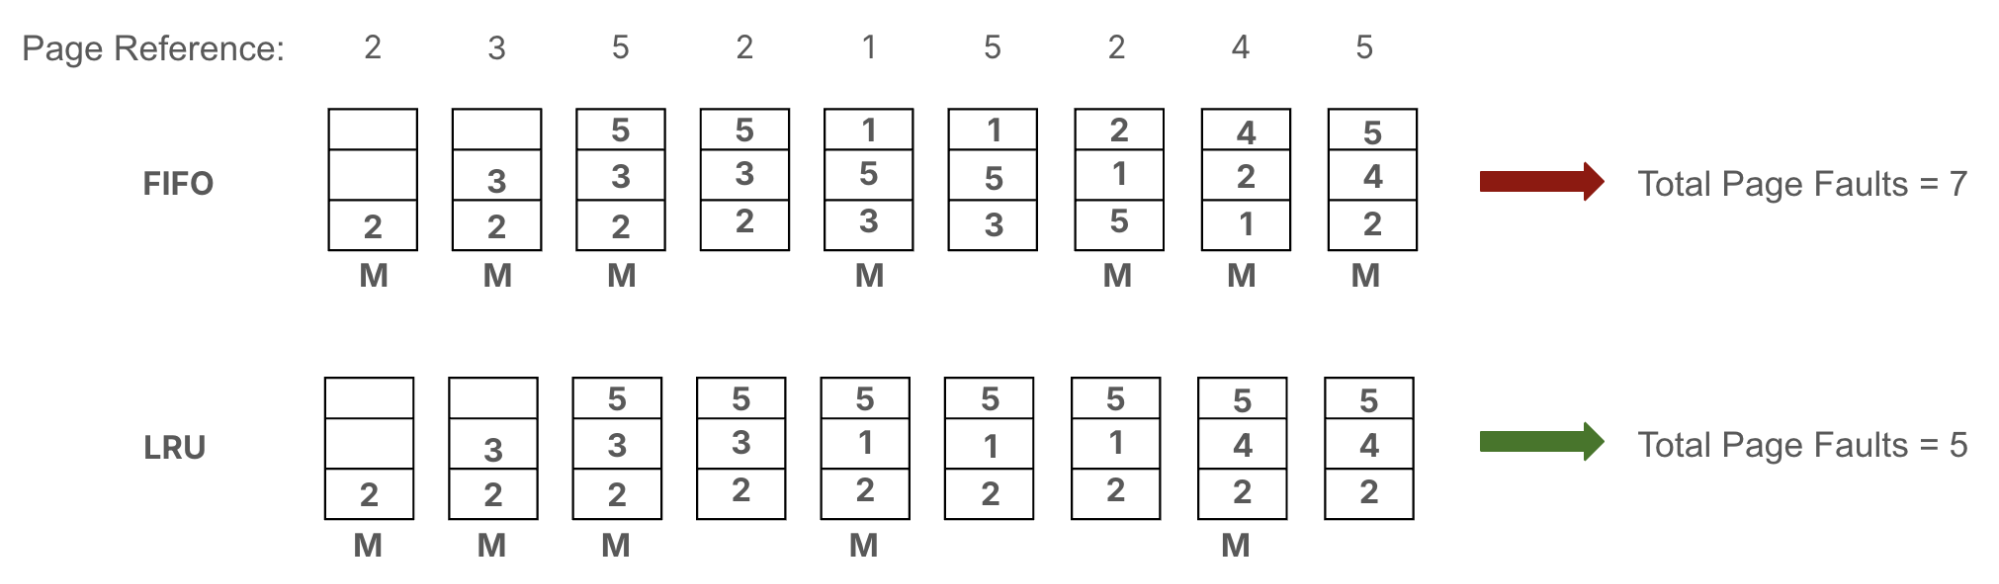
\includegraphics[width=0.85\textwidth]{fifo-vs-lru.png}
    \caption{FIFO vs.\ LRU eviction strategies.}
    \label{fig:fifo-lru}
\end{figure*}

\Cref{fig:fifo-lru} illustrates the fundamental difference between FIFO and
LRU eviction strategies in the KVM MMU. The FIFO approach removes the oldest page
in memory without considering its usage frequency, leading to unnecessary
evictions and increased page faults. In contrast, LRU keeps track of recently
accessed pages, ensuring that frequently used pages, such as page 2 and page 5,
remain in memory longer. As a result, LRU reduces the total number of page faults
(5) compared to FIFO (7), demonstrating its advantage in preserving memory
locality and minimizing costly page replacements. This aligns with our project's
goal of improving KVM's memory management efficiency by replacing FIFO with an
Approximate LRU mechanism.

\paragraph{Revision note.} The original version of this report described the
clock implementation only loosely and listed deadlocks and faults as unresolved.
We have since found two bugs in the eviction loop that explain them and fixed
both: a use-after-free, which we reproduced under KASAN, and an unbounded sweep,
which we found by reading the code. \Cref{sec:impl-clock,sec:impl-safety} describe the fixed design,
\cref{sec:validation} describes how we validated it, and the evaluation notes
which configuration each measurement came from.

\subsection{Scope and Objectives}

Given the importance of memory management in virtualization~\cite{waldspurger02}, our project focuses
on integrating an Approximate LRU eviction mechanism into KVM's MMU. Specifically,
our objectives were:

\begin{enumerate}[leftmargin=*,itemsep=2pt,topsep=2pt]
    \item \textbf{Design and Implement an LRU Eviction Policy:}
    \begin{itemize}[topsep=2pt,itemsep=1pt]
        \item Modify KVM's \textit{mmu.c} file to track page access recency and
              replace FIFO with LRU-based eviction logic.
        \item Adapt existing Linux kernel data structures to support an efficient
              Approximate LRU approach with minimal overhead.
    \end{itemize}

    \item \textbf{Validate Correctness Through Testing:}
    \begin{itemize}[topsep=2pt,itemsep=1pt]
        \item Use KVM unit tests and custom workloads to verify correctness and
              stability of the new eviction policy.
        \item Monitor page eviction patterns using kernel tracing tools such as
              tracepoints and Kprobes.
    \end{itemize}

    \item \textbf{Evaluate Performance Gains:}
    \begin{itemize}[topsep=2pt,itemsep=1pt]
        \item Measure page fault frequency, CPU utilization, and memory overhead
              using benchmarking tools.
        \item Compare the Approximate LRU implementation against FIFO to determine
              efficiency gains.
    \end{itemize}

    \item \textbf{Address Concurrency and Scalability:}
    \begin{itemize}[topsep=2pt,itemsep=1pt]
        \item Ensure the LRU eviction mechanism remains thread-safe in multi-CPU
              environments.
        \item Validate that the solution scales well under high-memory workloads.
    \end{itemize}
\end{enumerate}

\section{Related Works}

Before diving into our implementation, it is important to address related works.
Much of the prior research contrasting FIFO and LRU replacement policies is rooted
in both theoretical and practical investigations. Notably, ``It's Time to Revisit
LRU vs.\ FIFO'' highlights how large-scale caches, such as those in cloud object
storage, experience significant metadata overhead when implementing LRU. Because
storing and updating recency metadata can be expensive for massive caches, FIFO's
simpler management can sometimes produce less overhead~\cite{eytan2020}. This is an
important consideration for our work in cases where a large memory pool may affect
CPU overhead and latency.

On the other hand, a formal analysis conducted in ``LRU is Better Than FIFO''
underscores the fact that LRU outperforms FIFO in paging systems, especially when
workloads exhibit strong locality of reference. Their analysis results emphasize
the idea that retaining least recently used pages is beneficial for maintaining
``hot'' data in cache~\cite{chrobak1999, sleator1985}. This aligns with our project's objective
to integrate a more locality-aware eviction policy (LRU) into KVM's MMU. Although,
we must remain mindful of the potential overhead emphasized by ``It's Time to
Revisit LRU vs.\ FIFO''.

Additionally, it is important to note development work within the context of KVM
itself. The FIFO implementation of shadow page tables is a feature only used when
EPT hardware virtualization resources are not available within the environment.
Due to this, within most use cases, KVM uses a TDP MMU implementation that
leverages the given hardware, and is much more performant than shadow paging~\cite{bhargava2008}.
Thus, while our work may show performance benefits over the old implementation, it
is not a general improvement to the KVM project.

\section{Design Overview}

\subsection{System Architecture}

At a high level, our modified virtualization environment retains the existing KVM
framework, which provides the interface between guest virtual machines and host
hardware. KVM operates in kernel space, exposing virtualization extensions to a
user-space manager (e.g.\ QEMU) responsible for configuring virtual CPUs, devices,
and memory. Under the hood, KVM implements its own Memory Management Unit (MMU)
subsystem, managing page tables and address translations for each guest VM.

Our project inserts a custom eviction mechanism into this KVM MMU layer,
specifically within the page table code that decides when and how to replace
memory pages. The flow below outlines a simplified conceptual model of how KVM
handles virtualization and memory:

\begin{enumerate}[leftmargin=*,itemsep=2pt,topsep=2pt]
    \item Guest VMs issue memory operations (loads, stores), thinking they are
          running on real hardware.
    \item KVM traps these operations as needed, using the host CPU's
          virtualization capabilities.
    \item Page Table Structures in KVM's MMU track which guest pages are resident,
          which must be evicted, and handle faults.
    \item Host Kernel eventually services the page faults, interacting with actual
          RAM or swap.
\end{enumerate}

This flow is largely unchanged by our intervention except for the eviction logic,
which now uses an approximate LRU-based approach. By preserving the rest of the
hypervisor's design, we minimize disruption to the broader virtualization stack
while still providing a novel improvement in page eviction decisions.

\section{Implementation}

\subsection{Developer Environment Setup}

Our initial plan was to configure local development and run nested virtualization
for testing KVM. However, hardware limitations proved challenging: only one team
member had an x86 architecture laptop, while the others used Apple Silicon
(ARM-based) MacBooks. Since KVM is natively supported on x86 but not on ARM, we had
difficulties building and running custom kernels with KVM-enabled virtualization
locally. We also encountered setbacks with VirtualBox's nested virtualization.
Although theoretically supported, its performance and stability were inadequate
for continuous kernel development. To address these limitations, we first
experimented with UTM (Universal Turing Machine) on macOS, but it did not support
nested virtualization on Apple Silicon hardware. Next, we attempted to launch a
bare-metal AWS instance, discovering that the default plans available to us had
insufficient vCPU allocations. Eventually, after discussions with our course
instructor, we obtained access to a \texttt{c5n.metal} instance that met our
requirements. There, we set up a full Linux environment with KVM enabled, allowing
us to compile and debug custom kernel builds. On our one x86 laptop, we further
performed local tests and kernel compilations, though we had to re-partition the
Windows EFI space to accommodate larger kernels. All of this helped us establish a
consistent development workflow, merging and testing changes in an environment
representative of production KVM scenarios.

\subsection{Clock Eviction in the Shadow MMU}
\label{sec:impl-clock}

KVM's legacy (non-TDP) MMU keeps every shadow page in a per-VM list,
\texttt{kvm->arch.active\_mmu\_pages}. New pages go at the head, so the tail
holds the oldest. When fewer than 5 pages are free,
\texttt{make\_mmu\_pages\_available()} calls
\texttt{kvm\_mmu\_zap\_oldest\_mmu\_pages()} to free enough to get back to 25.
Upstream, that function walks the list from the tail and zaps the first
non-root pages it finds, which is FIFO.

Our change keeps the list and its order as they are and adds four things:
\begin{enumerate}[leftmargin=*,itemsep=2pt,topsep=2pt]
    \item \textbf{A reference bit per shadow page} (\texttt{sp->lru\_ref}). It
          is tracked per shadow page, not per page-table entry.
          \texttt{mark\_kvm\_page\_accessed()} sets it when
          \texttt{\_\_kvm\_mmu\_get\_shadow\_page()} looks up or creates the page,
          and when \texttt{fast\_page\_fault()} fixes a fault (or finds it
          spurious) through that page. \texttt{mmu\_set\_spte()} also sets it
          when it fills an SPTE in the page for a guest fault (not a
          prefetch), which we call \emph{marking on fill}.
    \item \textbf{A persistent clock hand} (\texttt{kvm->arch.clock\_hand}) that
          walks the list from oldest to newest and wraps around.
    \item \textbf{A new sweep}, \texttt{kvm\_mmu\_clock\_zap\_pages()}, used when
          the \texttt{kvm.lru\_mmu} module parameter is 1. At each page, the hand
          moves on first. Root pages are skipped. A page with its bit set gets
          the bit cleared and is skipped (its ``second chance''). Otherwise the
          page is zapped. The sweep stops once enough pages are freed.
    \item \textbf{Optional hardware accessed bits} (\texttt{kvm.lru\_age}).
          Mode 0, the default, is off. In mode 1 (\emph{leaf}) the sweep also
          tests and clears the hardware Accessed bit of every present SPTE in
          the page (up to 512), the way \texttt{kvm\_rmap\_age\_gfn\_range()}
          ages leaf SPTEs, and skips the page if any bit was set. In mode 2
          (\emph{parent}) it instead tests and clears the Accessed bit of the
          parent SPTE or SPTEs that point to the page, found through
          \texttt{sp->parent\_ptes}; the CPU sets that bit whenever a page walk
          passes through it. If a sweep clears Accessed bits but zaps nothing, it
          flushes the TLB so that cached translations set the bits again; a
          sweep that zaps already flushes. \Cref{sec:reuse} explains why this
          matters.
\end{enumerate}
Because pages are never moved, the list's FIFO order, which
\texttt{kvm\_zap\_obsolete\_pages()} depends on, still holds, and
\texttt{lru\_mmu=0} runs the upstream FIFO eviction loop unchanged. For experiments we also
added a \texttt{kvm.min\_alloc\_pages} parameter that caps each VM's shadow page
pool so eviction happens often. Its default, 0, keeps the upstream pool size; an
earlier version pinned every VM at 64 pages when the parameter was unset. Five
VM statistics count the sweep's work: \texttt{lru\_hand\_steps},
\texttt{lru\_ref\_skips}, \texttt{lru\_age\_sptes}, \texttt{lru\_age\_skips},
and \texttt{lru\_age\_flushes}. We also made \texttt{tdp\_mmu} and \texttt{ept}
writable so we could switch to the legacy MMU without rebooting.

\subsection{Thread Safety}
\label{sec:impl-safety}

We added no new locks. Every function that adds, removes, or zaps shadow pages
already holds \texttt{kvm->mmu\_lock} for writing, and so does the sweep. The
hand and the list are only changed under that lock, which lockdep now asserts.
Setting \texttt{lru\_ref} from the fast-fault path, which does not take the lock,
is a benign race: at worst a page gets one fewer second chance.

The first version of the sweep was not safe even under the lock, for two
reasons:
\begin{itemize}[leftmargin=*,itemsep=2pt,topsep=2pt]
    \item \textbf{A dangling hand.} Other paths also zap pages, such as deleting
          a memslot, which calls \texttt{kvm\_mmu\_zap\_all\_fast()}. If one of them
          freed the page the hand pointed to, the next sweep read freed memory.
          The fix is \texttt{kvm\_mmu\_clock\_hand\_unlink()}, called from
          \texttt{\_\_kvm\_mmu\_prepare\_zap\_page()}, which every zap path goes
          through. If the page leaving the list is under the hand, the hand
          moves to the next page first (or to \texttt{NULL} if the list is now
          empty). The sweep also moves the hand \emph{before} zapping, because a
          zap can remove other pages from the list too.
    \item \textbf{An unbounded loop.} If every page was a root or kept being
          re-referenced, the sweep never ended, and it spun while holding
          \texttt{mmu\_lock} for writing. We never reproduced a hang, but a spin like this
would look exactly like the deadlocks we saw. The
          fixed sweep has a budget of two laps
          ($2 \times$ \texttt{n\_used\_mmu\_pages} steps). The first lap clears
          every bit, so by the second lap any page that is not a root can be
          evicted. If the budget runs out, the caller gets back fewer pages than
          it asked for, which it already handles.
\end{itemize}

\subsection{Correctness Validation under Emulation}
\label{sec:validation}

The \texttt{c5n.metal} instance was no longer available when we fixed these bugs,
so we validated the fix on an x86 workstation without hardware nested
virtualization. We built the kernel with KASAN, lockdep
(\texttt{PROVE\_LOCKING}), \texttt{DEBUG\_LIST}, and \texttt{KVM\_PROVE\_MMU}
and booted it in QEMU's software emulator (TCG) with an emulated AMD CPU with
SVM. We loaded \texttt{kvm\_amd} with \texttt{npt=0}, so the guest page tables
really are shadowed, and ran the KVM selftests inside it with
\texttt{tdp\_mmu=0} and a small \texttt{min\_alloc\_pages} so eviction happens
constantly.

With the original code, \texttt{memslot\_modification\_stress\_test} triggers
\emph{``BUG: KASAN: slab-use-after-free in kvm\_mmu\_zap\_oldest\_mmu\_pages''},
where the freed page came from \texttt{kvm\_mmu\_zap\_all\_fast()}. This is the
dangling hand. With the fix, that test passes, and so do
\texttt{demand\_paging\_test}, \texttt{access\_tracking\_perf\_test},
\texttt{dirty\_log\_perf\_test}, and a 4-vCPU \texttt{mmu\_stress\_test},
including runs that switch \texttt{lru\_mmu} on and off between tests. Neither
KASAN nor lockdep reported anything.

These runs show correctness, not performance, because the emulator is orders of
magnitude slower than hardware. Soft lockups appeared in some multithreaded runs,
but they appeared with FIFO and with the TDP MMU too, so we attribute them to the
emulator. We did not test Intel VMX.

\section{Evaluation Methods / Results}

Our evaluation methodology focused on assessing the effectiveness of the
Approximate LRU implementation in improving memory efficiency, reducing page
faults, and maintaining low latency under load, all while minimizing performance
overhead. To achieve a comprehensive analysis, we used a combination of unit
testing with KVM's built-in test suite, synthetic memory stress testing with
\texttt{stress-ng}, performance profiling using flamegraphs~\cite{gregg2016}, and
application-level benchmarking with \texttt{redis-benchmark}. Key performance metrics included page
fault frequency, latency, CPU overhead, and request throughput (RPS).

All performance numbers below come from the \texttt{c5n.metal} runs of the
\emph{original} clock code, before the fixes in \cref{sec:impl-safety}. The fixes
change behavior only when the hand would have dangled or the sweep would have
run forever, so we expect the numbers to hold, but we have not re-measured them.
Most runs used \texttt{tdp\_mmu=0} with EPT still on. In that setup the legacy MMU
manages EPT tables for guest memory directly and does not shadow guest page
tables, so these runs exercise eviction but not full shadow paging.

\begin{figure*}[t]
    \centering
    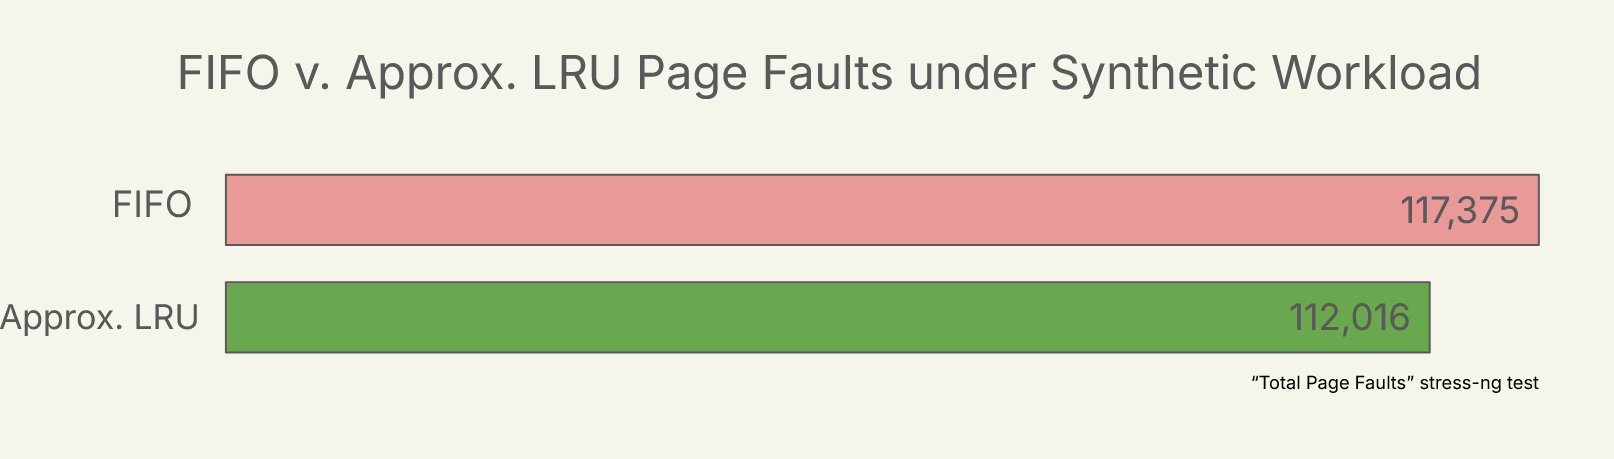
\includegraphics[width=0.8\textwidth]{page-faults.png}
    \caption{Page fault frequency comparison.}
    \label{fig:pagefaults}
\end{figure*}

One of the most direct indicators of improved memory management is page fault
frequency. Under stress testing with \texttt{stress-ng}, the traditional
FIFO eviction policy resulted in 117,375 page faults. In contrast, our
Approximate LRU implementation reduced this number to 112,016. This reduction
highlights more efficient memory reuse and fewer unnecessary page replacements.
Furthermore, performance profiling using flamegraphs revealed that Approximate LRU
led to fewer costly MMU interventions, supporting the claim of reduced overhead
and better memory locality. The difference is about 4.6\%, a modest improvement,
and we have no repeated runs to show how much it varies.

\begin{figure}[t]
    \centering
    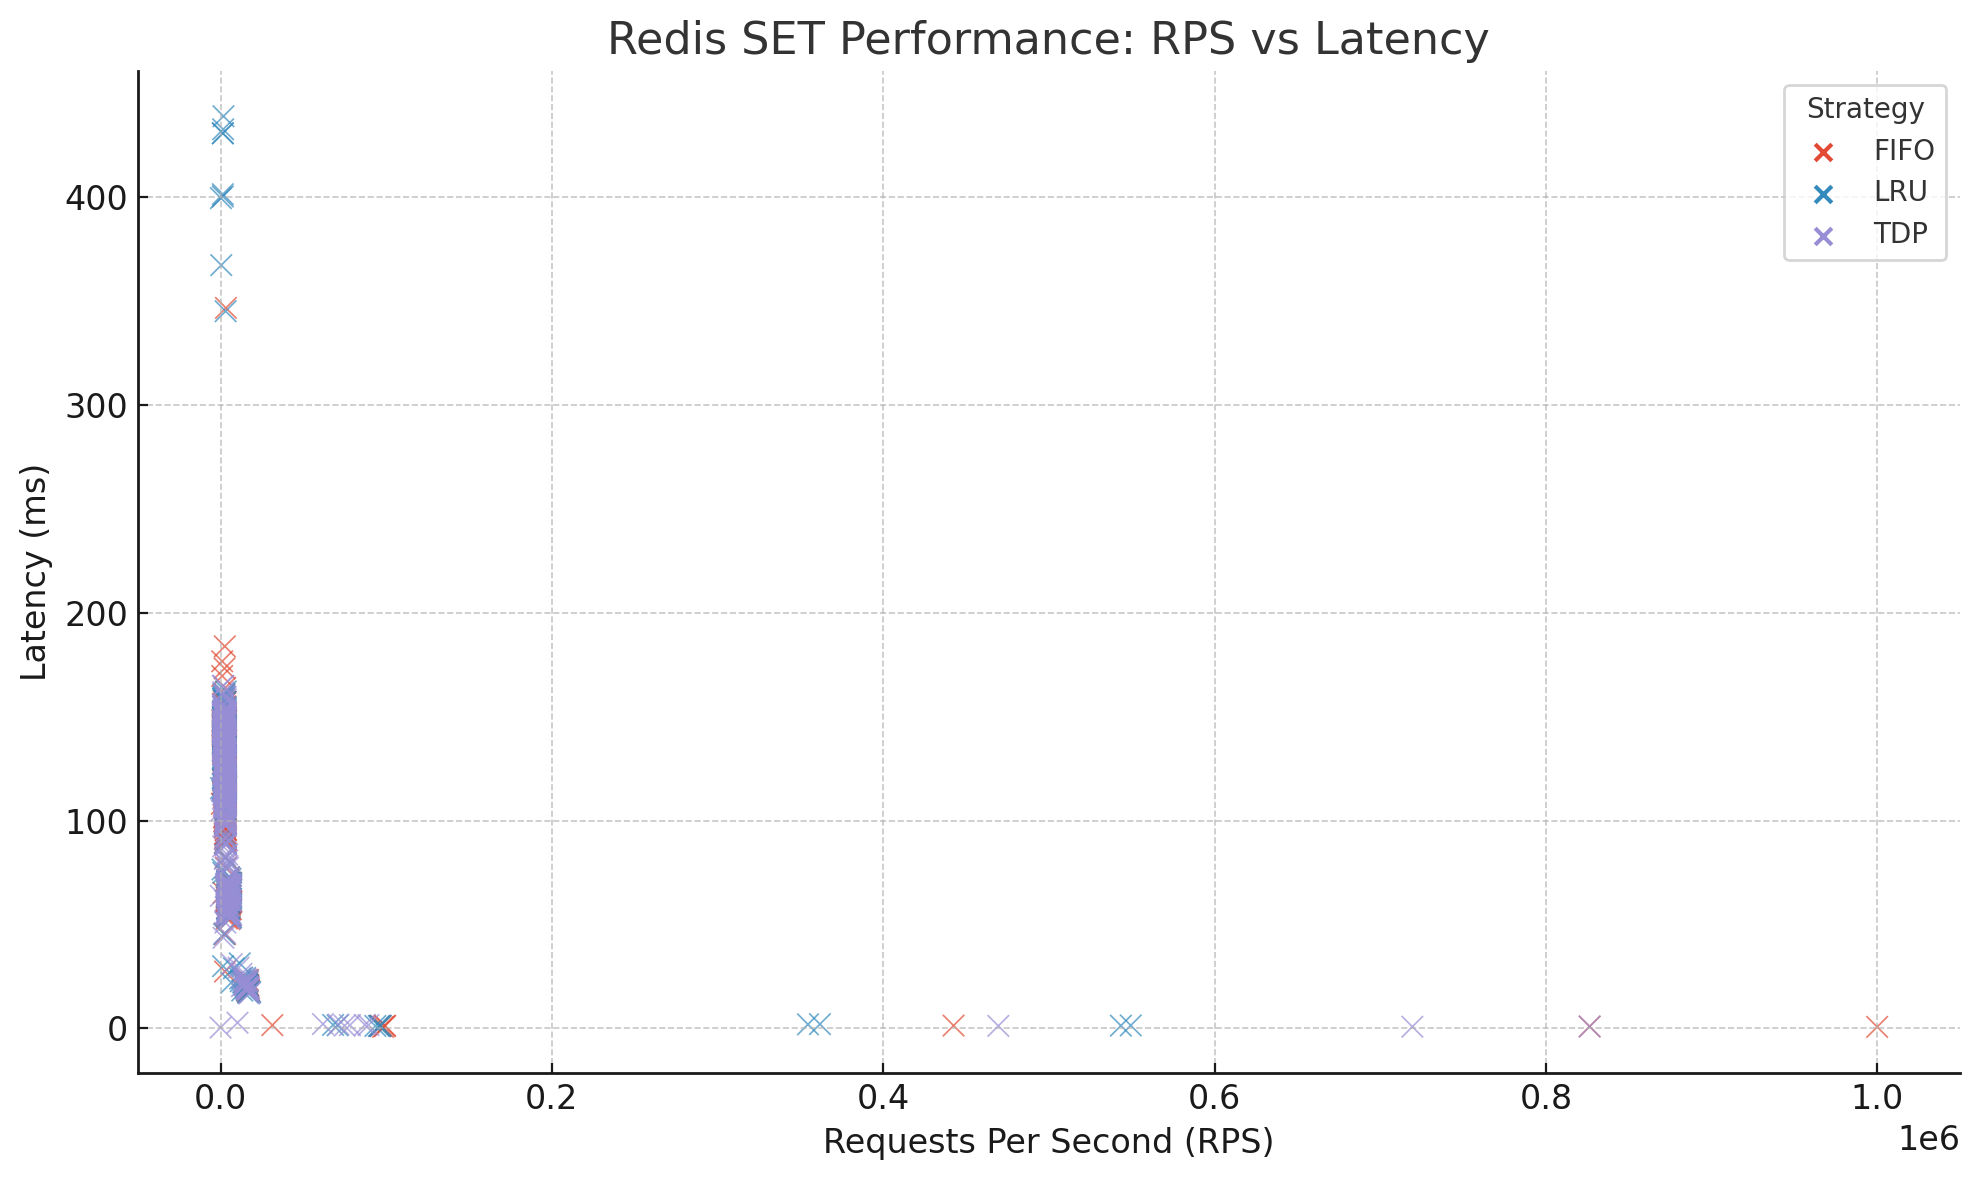
\includegraphics[width=\linewidth]{rps-vs-latency.png}
    \caption{RPS vs.\ latency for FIFO, LRU, and TDP.}
    \label{fig:rps-latency}
\end{figure}

Additionally, to evaluate real-world performance impact, we used the
\textit{redis-benchmark} tool, which simulates high-throughput client workloads.
The resulting graph shows the relationship between RPS and latency for three page
replacement strategies: FIFO, LRU, and TDP. LRU consistently delivers lower
latency across a wide range of RPS values, highlighting its efficiency in handling
frequent memory accesses. In contrast, FIFO exhibits increasing latency under
higher loads, indicating poor adaptability under stress. While TDP shows some
performance stability, it is more variable compared to LRU. Overall, this graph
suggests that our Approximate LRU implementation can sustain high throughput with
lower latency than FIFO. We treat the Redis results as suggestive only. They come
from single runs, and PING, which never reaches the eviction code, differed
between our FIFO and LRU runs by more than 30\% in both directions (one variant
faster, the other slower), so run-to-run noise is larger than the effect we are
looking for. Also, some of our Redis runs used an intermediate build in which
the calls that set \texttt{lru\_ref} were commented out, so the ``LRU'' in those
runs behaved like FIFO with a rotating start point. We have not been able to
confirm which build produced \cref{fig:rps-latency}.

\begin{figure*}[t]
    \centering
    \begin{subfigure}[t]{\textwidth}
        \centering
        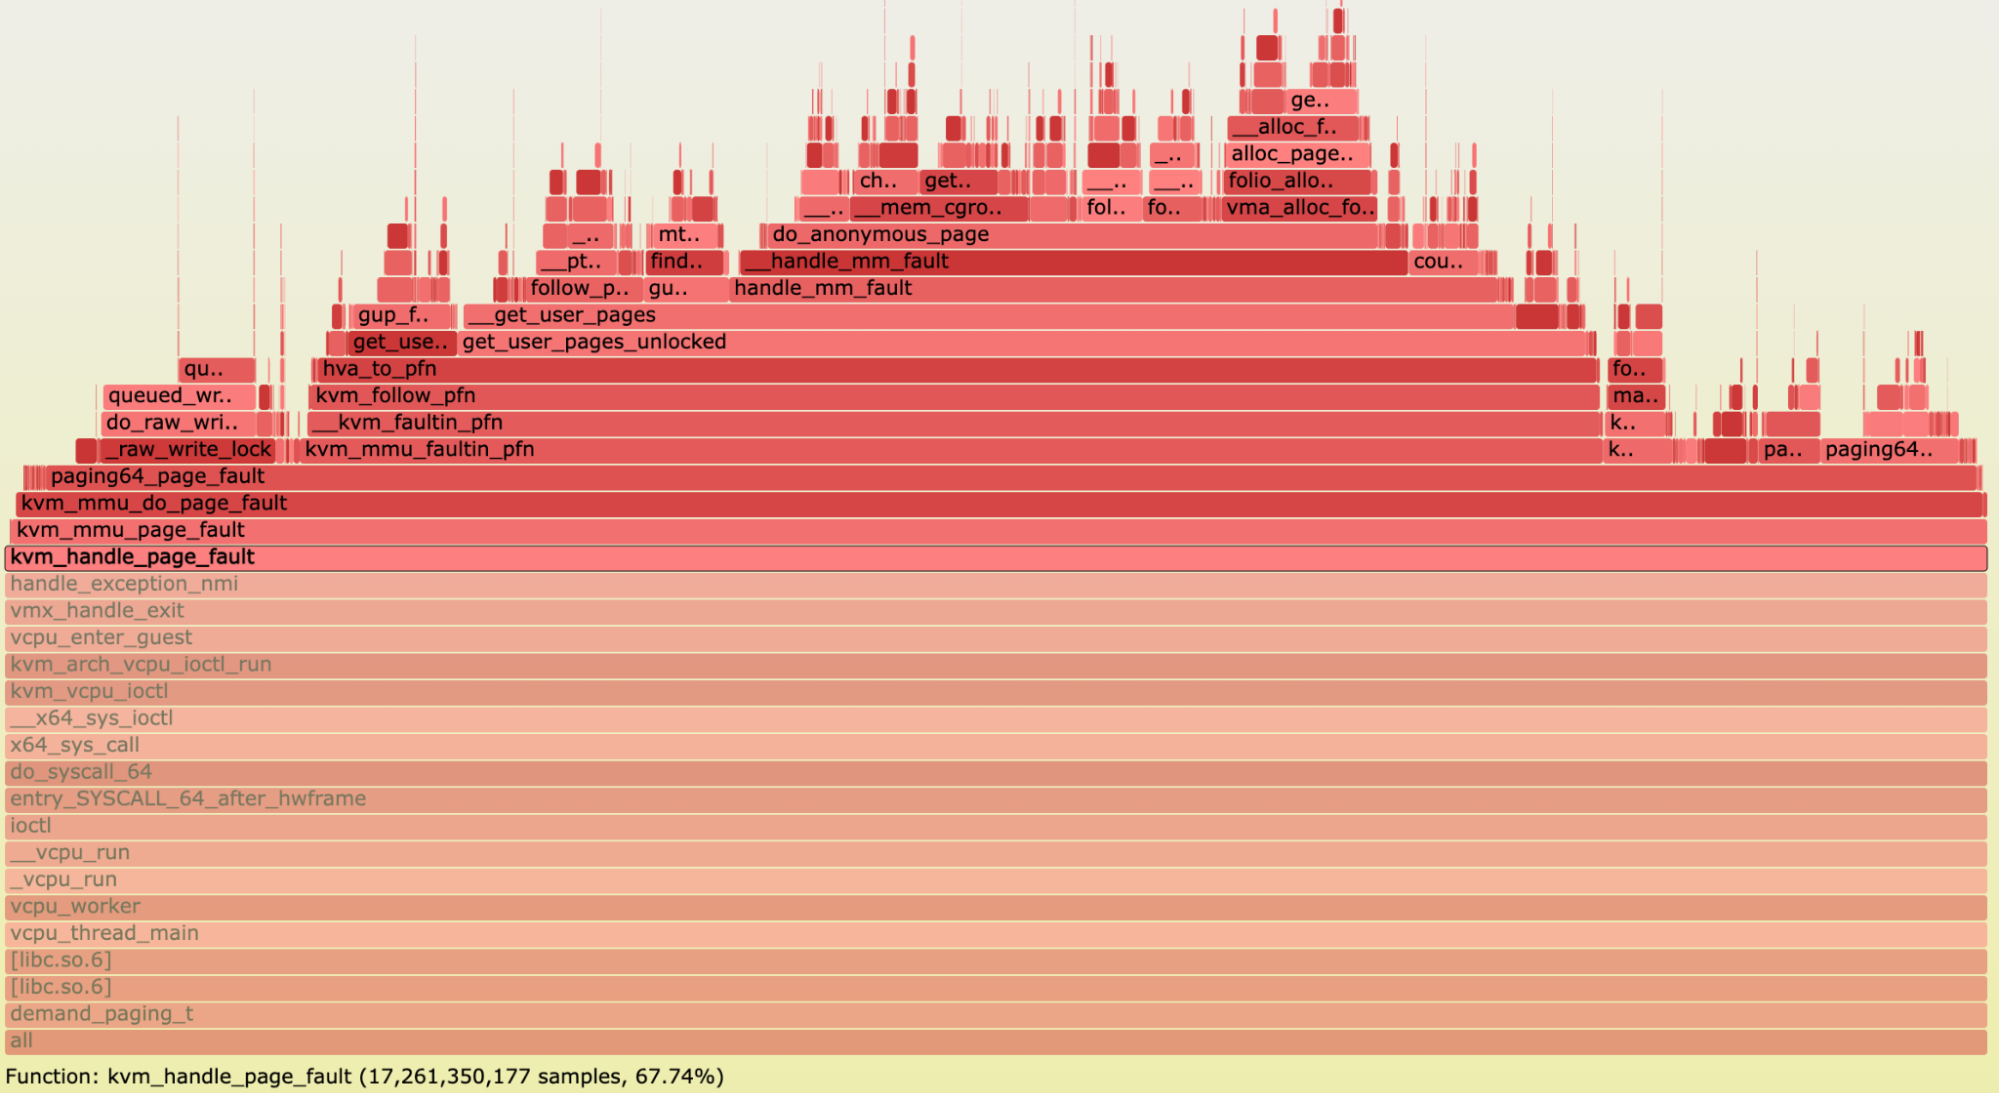
\includegraphics[width=0.92\linewidth]{flamegraph-fifo.png}
        \caption{FIFO.}
        \label{fig:flamegraph-fifo}
    \end{subfigure}

    \vspace{0.6em}

    \begin{subfigure}[t]{\textwidth}
        \centering
        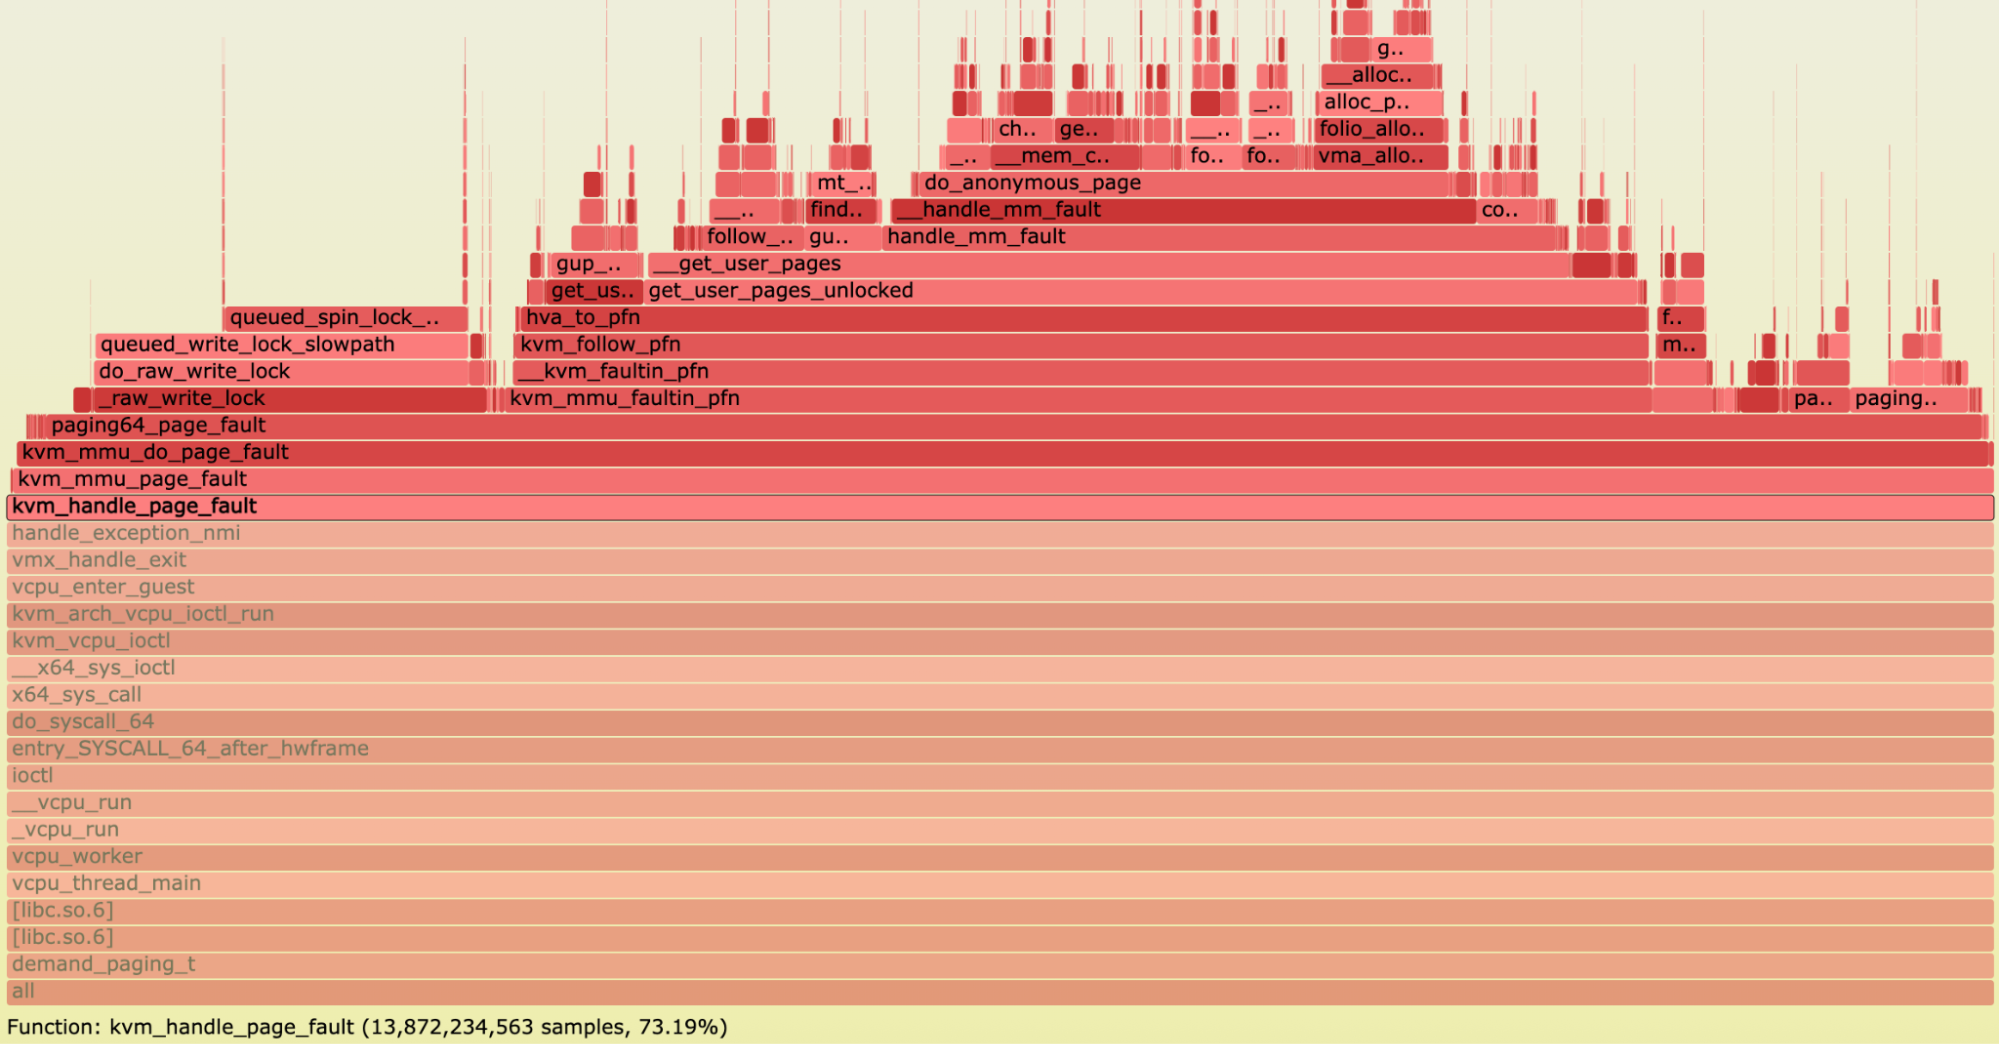
\includegraphics[width=0.92\linewidth]{flamegraph-lru.png}
        \caption{Approximate LRU.}
        \label{fig:flamegraph-lru}
    \end{subfigure}
    \caption{Flamegraphs of MMU page-fault handling under FIFO (top) versus
    Approximate LRU (bottom).}
    \label{fig:flamegraphs}
\end{figure*}

The evaluation of function-level performance highlights the impact of Approximate
LRU on page fault handling efficiency. As shown in \cref{fig:flamegraph-fifo},
key MMU functions, such as \texttt{kvm\_handle\_page\_fault} and
\texttt{kvm\_mmu\_page\_fault}, executed fewer times under Approximate LRU compared
to FIFO, indicating a reduction in overall page faults. Specifically, Approximate
LRU resulted in 3.39 billion fewer samples in
\texttt{kvm\_handle\_page\_fault}, demonstrating its ability to retain frequently
accessed pages and minimize unnecessary evictions. Similarly, the reduced relative
execution of \texttt{paging64\_page\_fault} and \texttt{kvm\_mmu\_faultin\_pfn}
methods suggests improved memory reuse, as fewer new pages needed to be loaded.
The presence of \texttt{paging64\_page\_fault} shows that this profile came
from a run with EPT disabled, where KVM shadows the guest's own page tables,
unlike the EPT-on runs described above.

However, while Approximate LRU reduces costly MMU interventions and improves memory
retention, CPU profiling revealed a slight increase in execution time for
MMU-related functions. This increase is attributed to the additional
overhead introduced by tracking page access recency. Consequently, although
Approximate LRU optimizes eviction decisions, it imposes a tradeoff between
efficiency and computational complexity. This tradeoff must be carefully considered
in scenarios where CPU overhead is a critical constraint. Nonetheless, the overall
reduction in page faults confirms that Approximate LRU enhances memory management
effectiveness compared to FIFO.

\subsection{Performance Comparison}

\begin{figure}[t]
    \centering
    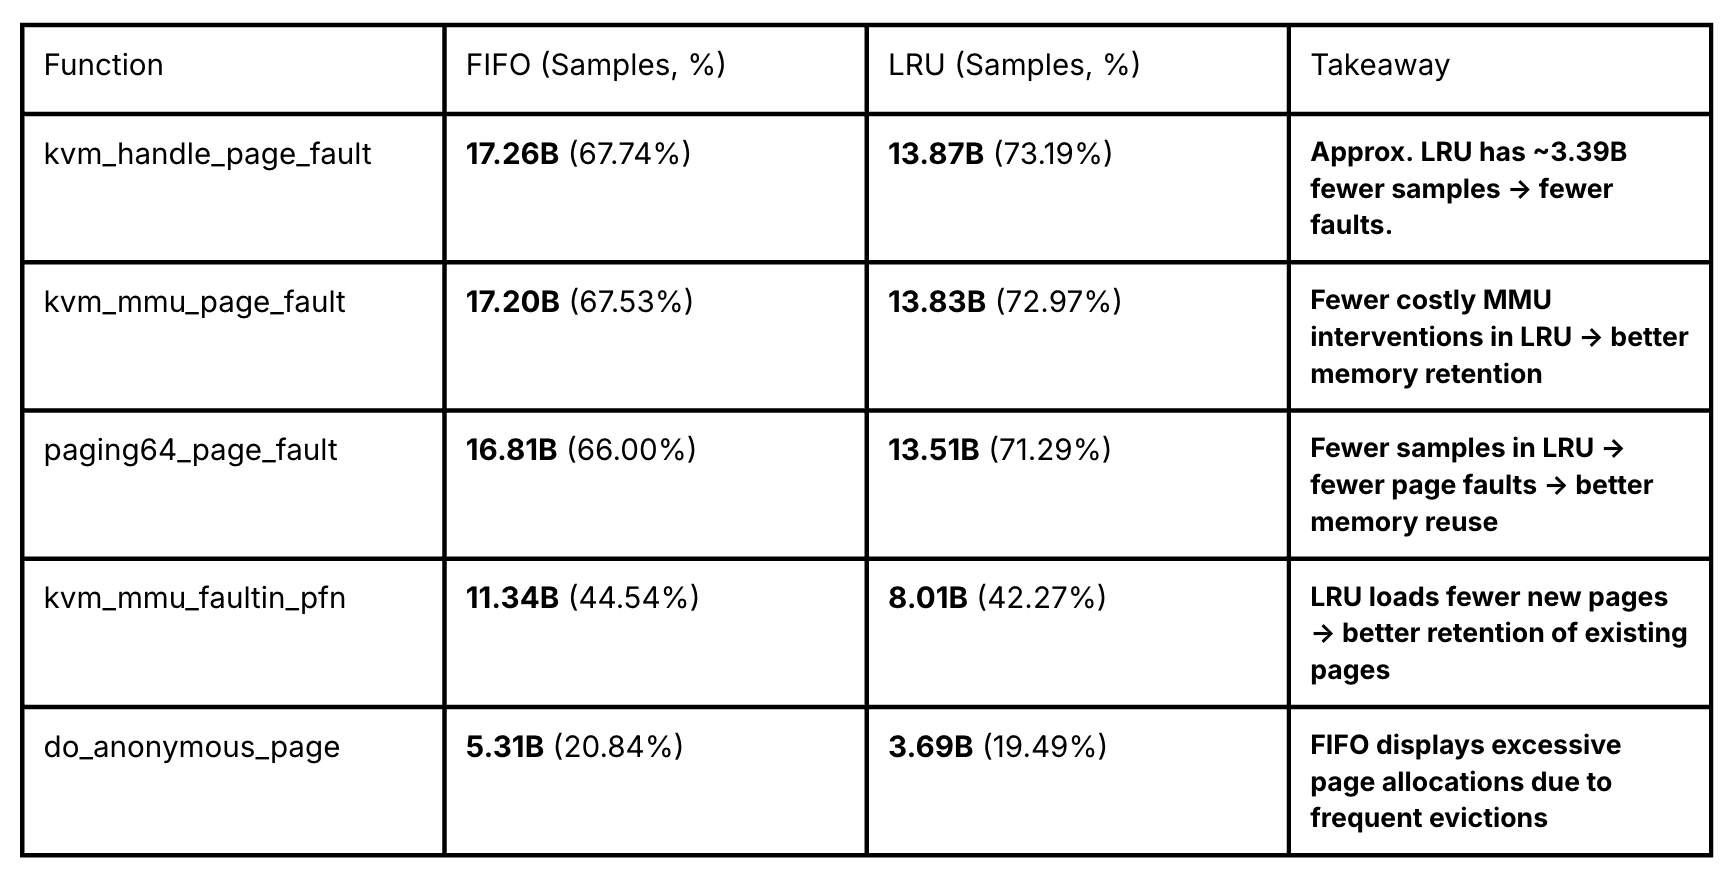
\includegraphics[width=\linewidth]{perf-comparison.png}
    \caption{Performance comparison summary.}
    \label{fig:perf-comparison}
\end{figure}

Overall, our evaluation confirmed that Approximate LRU successfully mitigates the
primary drawbacks of FIFO, reducing page faults and improving memory
locality at the cost of a slight increase in CPU processing. These findings
suggest that Approximate LRU offers a viable alternative to FIFO, particularly for
workloads that benefit from improved memory retention and reduced eviction churn.

\subsection{Eviction Counters with Reuse}
\label{sec:reuse}

The workloads above mostly sweep memory in order, which gives any recency policy
little to work with. To test a workload with reuse, we added a selftest,
\texttt{lru\_reuse\_test}. The guest touches 256 regions of 2\,MiB, each backed
by one last-level shadow page. Sixteen regions are hot and receive 90\% of the
accesses; the rest go to cold regions at random (\emph{hot}) or in order
(\emph{scan}). The trace depends only on a seed, so every policy sees the same
accesses. We ran it in the emulated setup of \cref{sec:validation}
(\texttt{npt=0}, \texttt{tdp\_mmu=0}) with 100{,}000 warm-up and 200{,}000
measured accesses, and report KVM's \texttt{pf\_taken} counter over the
measured phase, averaged over 3 seeds. The emulator makes timings meaningless,
so we report counters only.

The FIFO column and the ``marked on creation'' column come from the kernel
before \texttt{mmu\_set\_spte()} set \texttt{lru\_ref}; the other columns come
from the current kernel. The two are comparable: CLOCK with a 32-page pool on the
current kernel reproduces the earlier FIFO counts seed for seed. An earlier
version of this table reported larger \texttt{lru\_age} gains; those runs came
from a version of \texttt{lru\_reuse\_test} that overflowed its statistics
arrays, and we have replaced them.

\begin{table}[t]
    \centering
    \footnotesize
    \setlength{\tabcolsep}{4pt}
    \begin{tabular}{lrrrrrr}
        \hline
        Workload & Pool & FIFO & Create & Fill & Leaf & Parent \\
        \hline
        hot  & 32  & 212{,}854 & 0\%     & 0\%     & $-4\%$  & $-5\%$  \\
        hot  & 64  & 175{,}223 & $-11\%$ & $-61\%$ & $-55\%$ & $-82\%$ \\
        hot  & 128 & 119{,}108 & $+3\%$  & $-64\%$ & $-72\%$ & $-66\%$ \\
        scan & 32  & 213{,}098 & 0\%     & 0\%     & $-4\%$  & $-5\%$  \\
        scan & 64  & 179{,}150 & $-10\%$ & $-80\%$ & $-82\%$ & $-80\%$ \\
        scan & 128 & 143{,}191 & $-23\%$ & $-78\%$ & $-80\%$ & $-83\%$ \\
        \hline
    \end{tabular}
    \caption{Page faults in \texttt{lru\_reuse\_test} (mean of 3 seeds). CLOCK
    columns are relative to FIFO. \emph{Create}: \texttt{lru\_ref} set only
    when a shadow page is looked up or created. \emph{Fill}: also set on every
    non-prefetch SPTE fill. \emph{Leaf} and \emph{Parent}: Fill plus
    \texttt{lru\_age=1} or \texttt{lru\_age=2}.}
    \label{tab:reuse}
\end{table}

\Cref{tab:reuse} shows the result. When \texttt{lru\_ref} is set only on
creation, CLOCK is close to FIFO, and with a 32-page pool its counters match
FIFO's exactly. Once a shadow page exists, accesses through it are handled by
hardware and never exit to KVM, so a hot page's bit is set only when the page is
created, just like a cold page's. After one lap clears every bit, the sweep
evicts in FIFO order.

Marking on fill does most of the work. A guest that touches a new 4\,KiB page in
a region faults once to fill its SPTE, and the fill now sets the bit on the
shadow page that holds it. Hot regions keep taking such faults, so their pages
survive the sweep. This alone cuts faults by 61--80\% at pools of 64 and 128 and
zaps 11--30\% fewer shadow pages. The drop in faults exceeds the drop in zaps
because the pages kept are hot, and each zapped hot page costs a fault for every
4\,KiB page the guest touches again in its region.

The hardware Accessed bits add mixed gains on top. Parent mode has the fewest
faults in 4 of 6 rows and is never much worse than the best. Leaf mode is best
at hot/128 but worse than plain CLOCK at hot/64. At 32 pages, marking on fill
changes nothing, because the hot set barely fits, while both aging modes zap
23--24\% fewer pages and take 4--5\% fewer faults. Differences of a few points
between the CLOCK variants are within seed noise: plain CLOCK at hot/64 ranged
from 65{,}270 to 71{,}759 faults across seeds, parent mode at hot/128 from
36{,}234 to 48{,}134, and leaf mode at scan/128 from 23{,}853 to 38{,}077. The gap
to FIFO is well outside that noise.

The new statistics show the cost of aging. Leaf mode reads 1{,}145--1{,}352 SPTEs
per zapped page, since it checks up to 512 SPTEs in every page the hand passes.
Parent mode reads 1.2--2.3, since it checks only the parent SPTEs of each page.
The TLB flush after a sweep that
clears bits without zapping ran about 255--288 times per run at 32 pages and
almost never at 64 or 128. With the default pool size
(\texttt{min\_alloc\_pages=0}), this test zaps nothing and takes 34{,}728 faults
under both FIFO and CLOCK with parent mode, so the policy only matters when the
pool is under pressure.

Parent mode also leaves the leaf Accessed bits alone, which host reclaim reads
and clears through \texttt{kvm\_test\_age\_gfn()} and \texttt{kvm\_age\_gfn()};
leaf mode shares those bits with reclaim. As a check, we ran
\texttt{access\_tracking\_perf\_test} (4 vCPUs, 64\,MiB each, 64-page pool)
under FIFO, CLOCK, leaf, and parent mode. Every vCPU reported 0 of 16{,}384 pages
still idle, so no page was falsely reported idle, although the test was not
designed to catch interference from aging. We therefore recommend
\texttt{lru\_age=2} when \texttt{lru\_mmu=1}, but leave the default at 0 until
we have timings on real hardware.

In a workload that cycles through all regions in order (one seed, earlier
kernel), no policy helped by more than 7\%, and \texttt{lru\_age} was about 1\%
worse at 32 pages.

\section{Challenges}

\subsection{Difficulties Encountered}

Our initial challenges stemmed from environment setup and understanding the
existing codebase. A significant hurdle was establishing a development environment
compatible with KVM, particularly because many group members used Apple Silicon
MacBooks, necessitating an AWS bare-metal environment. This considerably extended
our development start time. Furthermore, comprehending the extensive KVM codebase
and the relatively large MMU codebase proved difficult. These two steps presented
substantial difficulties before we could begin implementing our changes. During
benchmarking and testing, we encountered stability issues, especially with larger
tests, which limited the workloads we could measure. We later found two bugs that
explain them, the dangling clock hand and the unbounded sweep, and fixed both
(\cref{sec:impl-safety}).

\subsection{What Didn't Work}

Our initial implementation revealed that the TDP MMU could not be optimized as
expected. Consequently, our analysis and optimization efforts focused on the older,
by-default-disabled shadow MMU. While our initial implementation on the existing
MMU was relatively swift, debugging and ensuring stability proved to be
significant challenges. Kernel crashes inside a nested guest gave us little to go
on. What finally located the bugs was a KASAN build, which pointed straight at the
freed page.

\subsection{What Did Work}

Our final implementation utilized a second-chance clock LRU
algorithm~\cite{corbato1968, ostep}, incorporating new functions for page tagging
and a per-VM clock hand. Once the hand was kept valid across every zap path and
the sweep was bounded, it passed the KVM selftests under KASAN and lockdep, and
the results indicate it reduces page faults compared to the previous FIFO MMU.

\section{Conclusion}

\subsection{Summary of Contributions}

In this project, we successfully implemented an Approximate LRU eviction policy to
replace the existing FIFO policy within the KVM Memory Management Unit (MMU). Our
modifications aimed to improve memory reuse, reducing page faults and enhancing
overall system efficiency. To validate our changes, we conducted extensive testing
in a controlled environment, using tracing, debugging, and benchmarking to analyze
system behavior. Our results confirmed eviction method tradeoffs. Notably,
approximate LRU reduces page faults and enhances memory efficiency, however FIFO
incurs a lower CPU overhead. The project code is available at:
\url{https://github.com/aaron-ang/kvm}.

\subsection{Future Extensions}

While our Approximate LRU implementation yielded positive results, there are
several directions for future improvement:

\begin{enumerate}[leftmargin=*,itemsep=2pt,topsep=2pt]
    \item \textbf{Re-measure on hardware:} Repeat the benchmarks with the fixed
          code, with EPT off, several runs per configuration, and a measured CPU
          overhead, and test on Intel VMX as well as AMD SVM.
    \item \textbf{Leaf mode and host reclaim:} Host reclaim reads the same
          leaf Accessed bits through \texttt{kvm\_test\_age\_gfn()} and clears
          them through \texttt{kvm\_age\_gfn()}. With \texttt{lru\_age=1}, the
          sweep and reclaim each clear bits the other relies on. Parent mode
          avoids this, and \texttt{access\_tracking\_perf\_test} found no
          falsely idle pages in either mode, but a test designed to provoke the
          interference would settle whether leaf mode is safe to use.
    \item \textbf{Timing the cost of aging:} The new statistics count the SPTEs
          each mode reads (about 1{,}300 per zap for leaf mode, about 2 for
          parent mode) and the TLB flushes it adds, but not how long they take
          under the write lock. Native timings would decide whether
          \texttt{lru\_age=2} should become the default.
    \item \textbf{Additional Benchmarking:} Evaluate the policy under a broader set
          of workloads and system configurations to ensure robustness across
          different environments.
    \item \textbf{Exploring Alternative Eviction Policies:} Compare the Approximate
          LRU with other eviction policies, such as hybrid FIFO-LRU or
          machine-learning-driven eviction mechanisms.
\end{enumerate}

\subsection{Reflection}

This project demonstrated the feasibility of improving KVM MMU memory management by
replacing FIFO with Approximate LRU. The process involved implementing the new
policy, validating it in controlled virtualized and cloud-based environments, and
analyzing its real-world performance. One of the key takeaways from this work is
the importance of balancing efficiency and overhead; while more sophisticated
eviction policies may further reduce page faults, they must remain lightweight to
avoid introducing performance bottlenecks. Additionally, the adaptability of
eviction strategies across different workloads remains an open challenge, making
ML-driven approaches an exciting avenue for future research. Overall, this work
contributes to the ongoing enhancement of KVM memory management, providing a
foundation for future research in eviction policies and performance optimization
in virtualized environments.

\balance
\begin{thebibliography}{10}

\bibitem{ostep}
Remzi H. Arpaci-Dusseau and Andrea C. Arpaci-Dusseau. \textit{Operating Systems:
Three Easy Pieces}. Arpaci-Dusseau Books, 1.00 edition, August 2018.

\bibitem{belady1966}
L.~A. Belady. A study of replacement algorithms for a virtual-storage computer.
\textit{IBM Systems Journal}, 5(2):78--101, 1966.

\bibitem{bhargava2008}
Ravi Bhargava, Benjamin Serebrin, Francesco Spadini, and Srilatha Manne.
Accelerating two-dimensional page walks for virtualized systems. In
\textit{Proceedings of the 13th International Conference on Architectural Support
for Programming Languages and Operating Systems (ASPLOS)}, pages 26--35, 2008.

\bibitem{chrobak1999}
Marek Chrobak and John Noga. LRU is better than FIFO. \textit{Algorithmica},
23:180--185, 1999. doi:10.1007/PL00009255.

\bibitem{corbato1968}
F.~J. Corbató. A paging experiment with the Multics system. In \textit{In Honor of
Philip M. Morse}, pages 217--228. MIT Press, 1969. (MIT Project MAC Memorandum
MAC-M-384, 1968.)

\bibitem{eytan2020}
Ohad Eytan, Danny Harnik, Effi Ofer, Roy Friedman, and Ronen Kat. It's time to
revisit LRU vs.\ FIFO. In \textit{Proceedings of the 12th USENIX Conference on Hot
Topics in Storage and File Systems (HotStorage '20)}, Article 12. USENIX
Association, 2020.

\bibitem{gregg2016}
Brendan Gregg. The flame graph. \textit{Communications of the ACM},
59(6):48--57, June 2016.

\bibitem{kivity2007}
Avi Kivity, Yaniv Kamay, Dor Laor, Uri Lublin, and Anthony Liguori. kvm: the Linux
virtual machine monitor. In \textit{Proceedings of the Linux Symposium}, volume~1,
pages 225--230, Ottawa, Canada, 2007.

\bibitem{sleator1985}
Daniel D. Sleator and Robert E. Tarjan. Amortized efficiency of list update and
paging rules. \textit{Communications of the ACM}, 28(2):202--208, 1985.
doi:10.1145/2786.2793.

\bibitem{waldspurger02}
Carl A. Waldspurger. Memory resource management in VMware ESX Server. In
\textit{Proceedings of the 5th Symposium on Operating Systems Design and
Implementation (OSDI)}, pages 181--194, 2002.

\end{thebibliography}

\end{document}
